\documentclass{report}

\usepackage{listings}
\usepackage{color}
\usepackage{graphicx}
\usepackage{float}

\begin{document}

\title{Image manipulation - in theoretical approach}

\author{Hamid Mirisaee,
\and Jander Nascimento, 
\and Raquel Oliveira}

\maketitle

\tableofcontents

\section{Image type}

	\subsection{PNG}

		\textit{Fill me}.

	\subsection{JPG}

		\textit{Fill me}.

	\subsection{GIF}

		\textit{Fill me}.

	\subsection{PNM}

		\textit{Fill me}.

\section{Filters}

	\subsection{Fundamental}

		By definition, a filter is a device or process which removes some unwanted features from an image (more precisely, form a signal).
		A low-pass(high-pass) filter is regarded as a classic example of filters in image processings area. Generally, filters are used to be convolved 
		(the convolution is described in the 
		next part) with an image in order to produce a new image. This new image, in turn, would be used for some other processings. The next subsection will
		intoduce the convolution and its basics.
		
		\subsubsection{Convolution}

			Convolutions are used to perform many useful image processing tasks such as noise reduction and edge detection. Generally,
			convolution is regardesd as a mathematical operation on two functions f and g which produces a modified version of one of the functions.
			Generally, but not necessarly, the first function (signal) is the input and is bigger than the second one.
			The following formula describes the continous convolution formula:
			
			
			When dealing with finite-length sequences, one cannot use the ordinary convolution formula (called linear convolution).
			In such cases, the circular convolution which results in zeros outside of the range of the signal is used. The mathematical formula of descrete 
			convolution could be seen in the following:
			
			In image processing field, basically, the image is the first function which is convolved with the second function, called kernel or filter.
			In this context we use the terms kernel and filter interchangably.
			There are a wide range of filters which are used to perform different tasks on a given image. The next subsection would go through some of these 
			filters which are used in the application in addition to a brief description for each.

		\subsection{Used filters}
		
		\subsubsection{Gaussian}

			The Gaussian kernel is a 2D convolution operator which is used to blur an image and remove noise. Mostly, applying a convolution using a Gaussian
			kernel is called Gaussioan smoothing.Generally, the Gaussian kernel is centered at
			zero (pick at 0). The following describes the Gaussian formula in 2D space:
			
			Gaussian smoothing acts almost the same as the mean filter, which will be in the following part.
		\subsubsection{Mean}
			Mean filter is an easy to implement kernel which is used to reduce the noise in an image by reducing the amount of intensity variation between one
			pixel and the next. The idea of the mean filter is to replace the value of each pixel with the average of its neighbors including itself. 
			
		
		\subsubsection{Gradient}

			\textit{Fill me}.
		




		\subsubsection{Laplacian}

			\textit{Fill me}.

\section{Color space}          

	\subsection{RGB}
		
		\textit{Fill me}.

	\subsection{CYMK}

		\textit{Fill me}.

	\subsection{Gray scale conversion}

		\textit{Fill me}.

\section{Cropping}

	\textit{Fill me}.

\section{Fusion}

	\textit{Fill me}.

\section{Resizing}

	Image resizing consist in convert an image to a size in which may or not respect the previous ratio.
	When dealing with reducing the size of an image is quite simple to do it, but when dealing with enlarging 
	the image, the process is a little bit complex.

	Reducing the dimension of an image consist in removing as many lines and as many columns as necessary to reach target dimension, of course this
	process may create some side-effect in the image, 

	When we stretch an image, we have few known pixels (dots which are image composition, think like the cells of a human being).

	There is a lot of algorithms that helps to guess (fill the gaps) those unknown pixels. for instance:

	\begin{itemize}
	  \item Nearest neighbor interpolation
	  \item Linear interpolation
	  \item Bilinear interpolation
	  \item Bicubic interpolation
	\end{itemize}

	The adopted algorithm is, \textbf{Bilinear interpolation},  due its speed and simplicity.
	
\subsection{From Linear to Bilinear interpolation}

	The Linear interpolation may be done horizontally or vertically, or even both. If a horizontal or vertical interpolation is done, we call it
	Linear interpolation, case both interpolations are applied its called Bilinear interpolation.	
	The pixel interpolation is done by calculating the mean of the known pixels around (vertical and horizontal axis) the unknown pixel. 


	\begin{figure} [H]
		\centering
		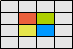
\includegraphics[scale=1]{images/bilinear_interpolation_1}
		\caption{original image \label{bilinear1}}
	\end{figure}

	On \ref{bilinear1} we can see the original image where all pixel are known pixels. Now what happen if we stretch this image 
	from a 2x2 to a 3x3\ref{bilinear2} image?
	
	\begin{figure} [H]
		\centering
		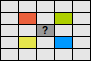
\includegraphics[scale=1]{images/bilinear_interpolation_2}
		\caption{original image \label{bilinear2}}
	\end{figure}

	As we can see, after stretch the image to a desired dimension we create some unknown pixels. To those pixels we can apply the Bilinear interpolation 
	to guess the color intensity we should use.

	Consider the values for the colors(c) red(r), green(g), blue(b) and yellow(y) respectively 20, 40, 60 and 80. The unknown pixel would be \[ f(?)=\frac{r+b}{2} + \frac{g+y}{2} \]

	This example is not realistic, because in most of the cases we must fill more than one gap in between known pixels. The same example in a more realistic way would be
	
	

\section{Histogram}

	\subsection{Color histogram}

		\textit{Fill me}.

	\subsection{Histogram stretching}

		\textit{Fill me}.

\end{document}
